\documentclass[11pt]{article}
\usepackage{amsmath, amsfonts, amsthm, amssymb}  % Some math symbols
\usepackage{enumerate}
\usepackage{fullpage}
\usepackage[x11names, rgb]{xcolor}
\usepackage{tikz}
\usepackage{graphicx}
\usetikzlibrary{snakes,arrows,shapes}
\usepackage{wasysym}
\usepackage{dsfont}
\usepackage{centernot}

\setlength{\parindent}{0pt}
\setlength{\parskip}{5pt plus 1pt}
\pagestyle{empty}

\def\indented#1{\list{}{}\item[]}
\let\indented=\endlist

\newcounter{questionCounter}
\newcounter{partCounter}[questionCounter]

\newenvironment{question}[2][\arabic{questionCounter}]{%
    \addtocounter{questionCounter}{1}%
    \setcounter{partCounter}{0}%
    \vspace{.25in} \hrule \vspace{0.5em}%
        \noindent{\bf #2}%
    \vspace{0.8em} \hrule \vspace{.10in}%
}{}

\renewenvironment{part}[1][\alph{partCounter}]{%
    \addtocounter{partCounter}{1}%
    \vspace{.10in}%
    \begin{indented}%
       {\bf (#1)} %
}{\end{indented}}

%%%%%%%%%%%%%%%%% Identifying Information %%%%%%%%%%%%%%%%%
%% This is here, so that you can make your homework look %%
%% pretty when you compile it.                           %%
%%     DO NOT PUT YOUR NAME ANYWHERE ELSE!!!!            %%
%%%%%%%%%%%%%%%%%%%%%%%%%%%%%%%%%%%%%%%%%%%%%%%%%%%%%%%%%%%
\newcommand{\myname}{Michael Rosenberg}
\newcommand{\myandrew}{mmrosenb@andrew.cmu.edu}
\newcommand{\mycourse}{73-449: Social, Economic, and Information Networks}
\newcommand{\myhwname}{| Final Project Proposal}
\newcommand{\myrecitation}{Anderson, Section A}
\newcommand{\myteammates}{}
\newcommand{\Z}{\mathds{Z}}
\newcommand{\bigdot}{\textbf{.} }
\newcommand{\spa}{\hspace{2cm}}
\newcommand{\proposition}{\textbf{\underline{Proposition:} }}
\newcommand{\proofwrite}{\textbf{\underline{Proof.} }}
\newcommand{\claim}{\textbf{\underline{Claim.} }}
\newcommand{\AFSOC}{Assume for the sake of contradiction }
\newcommand{\theorem}{\textbf{\underline{Theorem:}} }
\newcommand{\definition}{\textbf{\underline{Definition:}} }
\newcommand{\xNot}{\mathbf{x}_0}
%%%%%%%%%%%%%%%%%%%%%%%%%%%%%%%%%%%%%%%%%%%%%%%%%%%%%%%%%%%%%%%%%%%%%%%%%%%%%%%%

\begin{document}
\begin{center}
    {\Large \mycourse} {\Large \myhwname} \\
    \myrecitation \\
    \myname \\
    \myandrew \\
    %\myteammates 
\end{center}

For my final project, I will be doing an analysis of the Offshore Leaks
Database. This database shows relationships and networks among people and
companies in offshore entities that are traditionally designated as ``tax
havens''. Thus, to some degree, this database provides strong insights into how
the world's rich conduct offshore business. This database was constructed from
three leaks: the International Consortium of Investigative Journalists' (ICIJ)
China Leaks investigation in 2013, the Panama Papers leak in April 2016, and the
Bahamas Leak in September 2016.

Due to the size of the original network, I decided to start out my analysis by
only looking at behaviors within certain tax havens and certain Eastern
European countries. The visualization I have provided (see Figure 1) Contains
all agents associated with Russia, Ukraine, Poland, Panama, and The Bahamas and
all relationships among those agents.

This portion of the dataset contains $51336$ nodes (agents) and $39120$ edges
(relationships). The distribution of agents across country features $47.66\%$
from Panama, $31.48\%$ from Russia, $17.06\%$ from the Bahamas, $2.91\%$ from
Ukraine, and $0.88\%$ from Poland. When we look at the types of agents featured
in this subnetwork, $49.63\%$ of agents were entities (company created in
a tax haven), $27.33\%$ (person who plays a role in an entity), $20.35\%$ were
addresses (locations associated with agents), and $2.69\%$ were intermediaries
(go-betweens for entities and officers). Interestingly, despite the very
small portion of nodes being intermediaries, they play an extremely key role
in terms of degree in the network (see Figure 1). We see that the average
degree in this network is $1.524$, which suggests that this is a relatively
sparsely connected network. There are $16666$ weakly connected components in
the network, which suggests to me that to do further meaningful analyses on
this database, I will need to study all countries within the network due to the
apparent fragmentation that comes from studying only a couple of countries.
The clustering in this network is also relatively weak, as the average
clustering coefficient is $0.015.$ That being said, the network has an
average path length of $2.088$ in the largest connected component, which
suggests a potential small-world effect in the areas of the network that are
not severely fragmented.

Given the important place of intermediaries in the network, my question is
``are these intermediaries gaining social capital in this
network from brokerage or closure?'' There are two measures that will be
essential for studying this network. The first is the betweenness centrality
of intermediaries in the network, which will give me some measure of
brokerage associated with intermediaries. The second in average link
embeddedness for intermediaries in the network, which will give me a measure
of closure associated with intermediaries. I will make comparisons between these
two measures to study on average which of these are driving the importance of
intermediaries in this network. I will also make comparison between these
measures for intermediaries and these measures for other agents to ensure that
the brokerage/closure behavior of the intermediaries are significantly
different from that of entities and officers. These measures will give me a
strong sense as to what kind of social capital intermediaries have in this
network, and it will provide different policy implications as to how we might
want to sever gaps between officers and tax-haven entities.

\begin{figure}[h!]
    \centering
    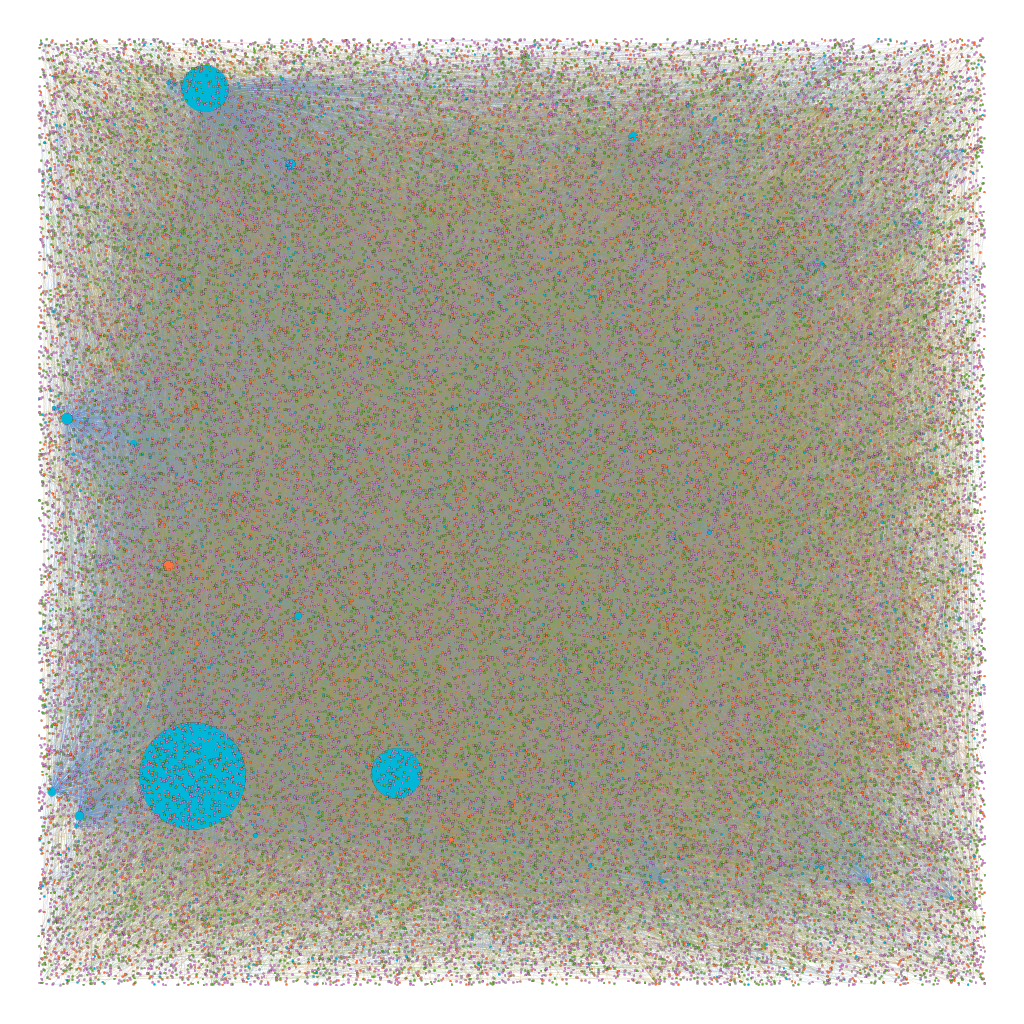
\includegraphics[width = 5in]{../analysis/figures/easternEuropeNetwork.png}
    \caption{Graph of our Eastern Europe network. The nodes are colored by
        agent type, where pink is for entities, green is for officers,
        orange is for addresses, and light blue is for intermediaries. Nodes
        are sized by degree.}
\end{figure}

\end{document}
